\documentclass[
11pt, % The default document font size, options: 10pt, 11pt, 12pt
codirector, % Uncomment to add a codirector to the title page
]{charter} 


% El títulos de la memoria, se usa en la carátula y se puede usar el cualquier lugar del documento con el comando \ttitle
\titulo{Sistema de monitoreo y gestión remota de red de sensores Bluetooth para el control del clima en invernaderos} 

% Nombre del posgrado, se usa en la carátula y se puede usar el cualquier lugar del documento con el comando \degreename
%\posgrado{Carrera de Especialización en Sistemas Embebidos} 
\posgrado{Carrera de Especialización en Internet de las Cosas} 
%\posgrado{Carrera de Especialización en Inteligencia Artificial}
%\posgrado{Maestría en Sistemas Embebidos} 
%\posgrado{Maestría en Internet de las cosas}
% IMPORTANTE: no omitir titulaciones ni tildación en los nombres, también se recomienda escribir los nombres completos (tal cual los tienen en su documento)
% Tu nombre, se puede usar el cualquier lugar del documento con el comando \authorname
\autor{Lic. Martín Anibal Lacheski}

% El nombre del director y co-director, se puede usar el cualquier lugar del documento con el comando \supname y \cosupname y \pertesupname y \pertecosupname
\director{Mg. Lic. Leopoldo Alfredo Zimperz}
\pertenenciaDirector{FIUBA} 
\codirector{Dra. Lic. Nancy Beatriz Ganz} % para que aparezca en la portada se debe descomentar la opción codirector en los parámetros de documentclass
\pertenenciaCoDirector{UNaM}

% Nombre del cliente, quien va a aprobar los resultados del proyecto, se puede usar con el comando \clientename y \empclientename
\cliente{Pablo Lodetti}
\empresaCliente{Wentux}
 
\fechaINICIO{20 de agosto de 2024}		%Fecha de inicio de la cursada de GdP \fechaInicioName
\fechaFINALPlan{8 de octubre de 2024} 	%Fecha de final de cursada de GdP
\fechaFINALTrabajo{23 de junio de 2025}	%Fecha de defensa pública del trabajo final


\begin{document}

\maketitle
\thispagestyle{empty}
\pagebreak


\thispagestyle{empty}
{\setlength{\parskip}{0pt}
	\tableofcontents{}
}
\pagebreak


\section*{Registros de cambios}
\label{sec:registro}


\begin{table}[ht]
	\label{tab:registro}
	\centering
	\begin{tabularx}{\linewidth}{@{}|c|X|c|@{}}
		\hline
		\rowcolor[HTML]{C0C0C0}
		Revisión & \multicolumn{1}{c|}{\cellcolor[HTML]{C0C0C0}Detalles de los cambios realizados} & Fecha                       \\ \hline
		0        & Creación del documento                                                          & \fechaInicioName            \\ \hline
		1        & Se completa hasta el punto 5 inclusive                                          & {2} de {septiembre} de 2024 \\ \hline
		%2      & Se completa hasta el punto 9 inclusive
		%		  Se puede agregar algo más \newline
		%		  En distintas líneas \newline
		%		  Así                                                    & {día} de {mes} de 202X \\ \hline
		%3      & Se completa hasta el punto 12 inclusive                & {día} de {mes} de 202X \\ \hline
		%4      & Se completa el plan	                                 & {día} de {mes} de 202X \\ \hline

		% Si hay más correcciones pasada la versión 4 también se deben especificar acá
	\end{tabularx}
\end{table}

\pagebreak



\section*{Acta de constitución del proyecto}
\label{sec:acta}

\begin{flushright}
	Buenos Aires, \fechaInicioName
\end{flushright}

\vspace{2cm}

Por medio de la presente se acuerda con el \authorname\hspace{1px} que su Trabajo Final de la \degreename\hspace{1px} se titulará ``\ttitle'' y
consistirá en {desarrollar un prototipo preliminar de un sistema basado en una red de sensores y actuadores inalámbricos, junto con un servidor en la nube y
		una aplicación web, que permita el monitoreo y control remoto del clima en invernaderos}.

El trabajo tendrá un presupuesto preliminar estimado de \textcolor{red}{600} horas y un costo estimado de \textcolor{red}{\$ XXX},
con fecha de inicio el \fechaInicioName\hspace{1px} y fecha de presentación pública el \fechaFinalName.

Se adjunta a esta acta la planificación inicial.

\vfill

% Esta parte se construye sola con la información que hayan cargado en el preámbulo del documento y no debe modificarla
\begin{table}[ht]
	\centering
	\begin{tabular}{ccc}
		\begin{tabular}[c]{@{}c@{}}Dr. Ing. Ariel Lutenberg \\ Director posgrado FIUBA\end{tabular} & \hspace{2cm} &
		\begin{tabular}[c]{@{}c@{}}\clientename \\ \empclientename \end{tabular} \vspace{2.5cm}                      \\
		\begin{tabular}[c]{@{}c@{}}\supname \\ Director del Trabajo Final\end{tabular}              & \hspace{2cm} &
		\begin{tabular}[c]{@{}c@{}}\cosupname \\ Codirectora del Trabajo Final \end{tabular} \vspace{2.5cm}          \\
		%\multicolumn{3}{c}{\begin{tabular}[c]{@{}c@{}} \supname \\ Director del Trabajo Final\end{tabular}} \vspace{2.5cm} \\
	\end{tabular}
\end{table}




\section{1. Descripción técnica-conceptual del proyecto a realizar}
\label{sec:descripcion}

La agricultura enfrenta desafíos crecientes en la optimización de la productividad y la eficiencia, especialmente en regiones con condiciones
climáticas adversas y variables. Los sistemas de cultivo tradicionales suelen ser ineficientes en la gestión de recursos esenciales como agua,
nutrientes y energía, en gran parte debido a la falta de monitoreo en tiempo real, lo que afecta negativamente tanto la calidad como el rendimiento
de los cultivos. Además, los agricultores se enfrentan a altos costos operativos y a un impacto negativo en la sostenibilidad ambiental debido a
prácticas no optimizadas. Ante estas dificultades, los cultivos en invernaderos han surgido como una solución mejorada, permitiendo un mayor
control sobre las condiciones ambientales y una utilización más eficiente de los recursos.


Este trabajo se desarrolla en colaboración con Wentux, una empresa argentina que, desde 2018, se dedica al desarrollo de soluciones tecnológicas basadas en
IoT (\textit{Internet of Things}) para la gestión del clima en invernaderos. La iniciativa surge a partir del programa de vinculación con empresas del posgrado,
que busca fomentar la colaboración entre el sector académico y el ámbito empresarial. Wentux ofrece productos que permiten controlar de manera automatizada
el clima de los cultivos mediante el uso de sensores y actuadores.


Actualmente, los sistemas de Wentux están compuestos por un nodo central con conexión Wi-Fi y sensores y actuadores conectados de forma cableada, lo cual
limita la flexibilidad y escalabilidad de la solución. Los datos del sistema se visualizan a través de una página web integrada en el nodo central,
y el monitoreo y control se realizan únicamente de manera local.


La propuesta, como puede observarse en la figura \ref{fig:diagBloques}, consiste en desarrollar una red Mesh (malla) de sensores y actuadores inalámbricos
basados en el ESP32-C3, que se conectan a un módulo central mediante tecnología BLE (\textit{Bluetooth Low Energy}). Este módulo, también basado en un ESP32-C3,
se conecta a Internet vía Wi-Fi y envía los datos a un servidor IoT a través del protocolo MQTT (\textit{Message Queue Telemetry Transport}). Esto permitirá
monitorear y gestionar el sistema de manera remota desde una aplicación web del tipo SPA (\textit{Single Page Application}).

\begin{figure}[htpb]
	\centering
	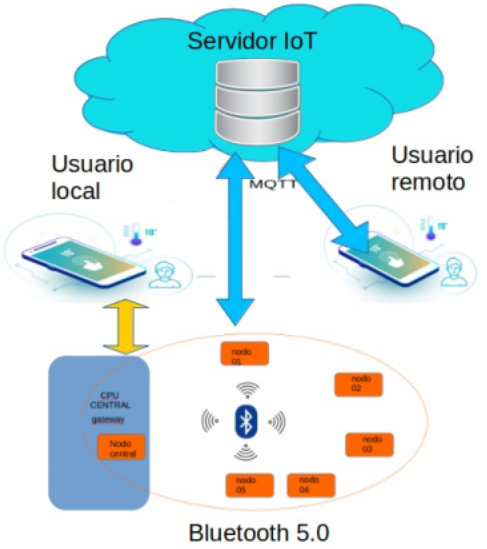
\includegraphics[width=.85\textwidth]{./Figuras/figura1.png}
	\caption{Diagrama en bloques del sistema.}
	\label{fig:diagBloques}
\end{figure}


Esta solución ofrece a los clientes finales un mayor control sobre sus cultivos, mejora la eficiencia en la gestión del clima y
optimiza los recursos, lo que se traduce en una mayor productividad y una reducción de los costos operativos.


\section{2. Identificación y análisis de los interesados}
\label{sec:interesados}

\begin{table}[ht]
	%\caption{Identificación de los interesados}
	%\label{tab:interesados}
	\begin{tabularx}{\linewidth}{|p{2.15cm}|p{5.8cm}|p{2.1cm}|p{4.1cm}|}
		\hline
		\rowcolor[HTML]{C0C0C0}
		Rol                           & Nombre y Apellido                                                                              & Organización    & Puesto              \\ \hline
		Cliente                       & \clientename                                                                                   & \empclientename & Responsable técnico \\ \hline
		Responsable                   & \authorname                                                                                    & FIUBA           & Alumno              \\ \hline
		\multirow{2}{*}{Orientadores} & \supname                                                                                       & \pertesupname   & Director            \\
		                              & \cosupname                                                                                     & \pertecosupname & Codirectora         \\ \hline
		Opositores                    & \multicolumn{3}{l|}{Empresas que ya ofrecen soluciones similares en el mercado.}                                                       \\ \hline
		Usuario final                 & \multicolumn{3}{l|}{Potenciales clientes interesados en automatizar cultivos en invernaderos.}                                         \\ \hline
	\end{tabularx}
\end{table}

\begin{itemize}
	\item Cliente: El señor \clientename\hspace{1px} tiene amplios conocimientos en desarrollo de sistemas embebidos y va a colaborar con la definición
	      de los requerimientos, el apoyo financiero y el seguimiento del proyecto.
	\item Orientadores:
	      \begin{itemize}
		      \item El Director \supname\hspace{1px} es experto en la temática y guiará con la implementación de los protocolos y herramientas del proyecto.
		      \item La Codirectora \cosupname , experta en Sistemas de Información, ayudará con el seguimiento metodológico, para garantizar una gestión
		            rigurosa y efectiva del desarrollo del trabajo.
	      \end{itemize}
\end{itemize}


\section{3. Propósito del proyecto}
\label{sec:proposito}

Diseñar y desarrollar un prototipo preliminar de una red en malla de sensores y actuadores inalámbricos conectados a través de BLE, junto con un servidor
IoT y una aplicación web, que permita el monitoreo y control remoto del clima en invernaderos. El proyecto busca proporcionar a los agricultores un mayor
control sobre las condiciones  ambientales, optimizar el uso de recursos, reducir los costos operativos y contribuir a una mayor sostenibilidad ambiental.

\section{4. Alcance del proyecto}
\label{sec:alcance}

El presente trabajo incluye:
\begin{itemize}
	\item Análisis e investigación de ESP-BLE-MESH para microcontroladores ESP32-C3.
	\item Implementación del protocolo ESP-BLE-MESH entre los nodos sensores, actuadores y el nodo central.
	\item Diseño e implementación de la conexión WiFi en el nodo central.
	\item Desarrollo del firmware de los nodos que serán alimentados con fuente 12vcc.
	      \begin{itemize}
		      \item Programación del firmware de los siguentes nodos sensores para la recopilación y transmisión de datos.
		            \begin{itemize}
			            \item Nodo sensor de temperatura ambiente y humedad relativa.
			            \item Nodo sensor de dióxido de carbono ($CO_2$).
			            \item Nodo sensor de potencial de hidrógeno (pH).
			            \item Nodo sensor de conductividad eléctrica (CE).
		            \end{itemize}
		      \item Programación del firmware del nodo actuador de cuatro salidas para gestionar el control de dispositivos y reportar su estado.
		      \item Programación del firmware del nodo central para gestionar la comunicación con los nodos sensores, actuadores y el servidor IoT.
		            \begin{itemize}
			            \item Programación del firmware del ESP32-C3 que actúa como nodo central en la topología mesh mediante Bluetooth (ESP-BLE-MESH).
			            \item Programación del firmware del ESP32-C3 que opera el servidor web y gestiona la comunicación con el servidor IoT mediante WiFi.
			            \item Programación del firmware para la comunicación entre los dos ESP32-C3 mediante UART (\textit{Universal Asynchronous Receiver-Transmitter}).
		            \end{itemize}
	      \end{itemize}
	\item Implementación del broker MQTT en el servidor IoT.
	\item Implementación de cifrados de conexión mediante TLS (\textit{Transport Layer Security}).
	\item Configuración del nodo central para enviar los datos recolectados al servidor IoT mediante el protocolo MQTT.
	\item Diseño e implementación de una base de datos para almacenar los datos recolectados por los sensores y permitir su consulta y análisis.
	\item Diseño y desarrollo de una API (\textit{Application Programming Interface}) REST (\textit{Representational State Transfer}) que permita la comunicación
	      con el sistema utilizando HTTP (\textit{Hypertext Transfer Protocol}), MQTT y WebSockets.
	\item Desarrollo de una aplicación Web SPA.
	\item Entrega del código del sistema, que incluye todos los componentes desarrollados (sensores, nodo central, servidor
	      y aplicación web), guías de instalación, configuración y operación.
\end{itemize}

El presente trabajo no incluye:
\begin{itemize}
	\item Diseño de los gabinetes para los nodos sensores, actuadores y nodo central a utilizar.
	\item Desarrollo de una aplicación móvil compatible con iOS y Android.
	\item Desarrollo de módulos para alimentación con baterías.
\end{itemize}



\section{5. Supuestos del proyecto}
\label{sec:supuestos}

Para el desarrollo del presente proyecto se supone que:

\begin{itemize}
	\item Se contará con los materiales necesarios para la implementación de los nodos de sensores, actuadores, como así también del nodo central.
	\item Se contará con el apoyo financiero del cliente para comprar los componentes adicionales necesarios para el desarrollo del prototipo.
	\item Se dispondrá del conocimiento necesario para la implementación del protocolo BLE Mesh en los microcontroladores.
	\item Se dispondrá del conocimiento necesario para la implementación del protocolo de cifrado TLS y el software necesario en los microcontroladores y servidor IoT.
	\item Se dispondrá del conocimiento necesario para el diseño y desarrollo de la base de datos, API y la aplicación SPA.
	\item El cliente tendrá disponibilidad para atender las consultas.
	\item Los directores tendrán disponibilidad para atender las consultas.
	\item Se podrá terminar el presente proyecto en el tiempo estipulado.
\end{itemize}

\section{6. Requerimientos}
\label{sec:requerimientos}

\begin{enumerate}
	\item Requerimientos de los nodos sensores:
	      \begin{enumerate}
		      \item Cada nodo deberá contar con un microcontrolador ESP32-C3.
		      \item Cada nodo deberá conectarse a una red Mesh sobre Bluetooth LE (Bluetooth 5).
		      \item Cada nodo deberá tener un identificador único dentro del sistema.
		      \item Cada nodo deberá permitir configurar el tiempo de manera remota para enviar los datos recolectados.
		      \item Cada nodo, según corresponda, deberá enviar al nodo central:
		            \begin{enumerate}
			            \item la temperatura del ambiente y humedad relativa,
			            \item el nivel de dióxido de carbono,
			            \item el nivel de pH y
			            \item y el nivel de CE.
		            \end{enumerate}
	      \end{enumerate}

	\item Requerimientos del nodo actuador:
	      \begin{enumerate}
		      \item Deberá contar con un microcontrolador ESP32-C3.
		      \item Deberá conectarse a una red Mesh sobre Bluetooth LE (Bluetooth 5).
		      \item Deberá tener un identificador único dentro del sistema.
		      \item Deberá contar con cuatro canales.
		      \item Deberá enviar al nodo central el estado de cada canal.
		      \item Deberá permitir activar cada canal de manera remota.
	      \end{enumerate}

	\item Requerimientos del nodo central:
	      \begin{enumerate}
		      \item Deberá contar con dos microcontroladores ESP32-C3.
		            \begin{enumerate}
			            \item Gateway de Red Mesh BLE
			            \item Servidor Web y conexión WiFi
		            \end{enumerate}
		      \item La comunicación entre ambos microcontroladores deberá ser realizada por UART.
		      \item Deberá procesar la información recibida de los nodos sensores y el nodo actuador.
		      \item Deberá enviar configuraciones y acciones a los nodos sensores y el nodo actuador.
	      \end{enumerate}

	      \pagebreak

	\item Requerimientos asociados al Gateway de Red Mesh BLE:
	      \begin{enumerate}
		      \item Deberá conectarse a una red Mesh sobre BLE y actuar como gateway de la red.
		      \item Deberá recibir los datos de los nodos sensores y del nodo actuador.
		      \item Deberá procesar y enviar la información al Servidor Web y conexión WiFi mediante UART.
		      \item Deberá gestionar los identificadores únicos de cada nodo de la red Mesh BLE.
	      \end{enumerate}

	\item Requerimientos asociados al Servidor Web y conexión WiFi:
	      \begin{enumerate}
		      \item Deberá poder conectarse a una red WiFi disponible.
		      \item Deberá poseer una página web embebida para monitoreo y configuración del sistema de manera local.
		      \item Deberá recibir la información del Gateway de Red Mesh BLE mediante UART.
		      \item Deberá enviar parámetros y acciones a los nodos sensores y actuadores a través del Gateway de Red Mesh BLE mediante UART.
		      \item Deberá enviar los datos al servidor IoT a través del protocolo MQTT.
		      \item Deberá implementar TLS para garantizar la seguridad en la comunicación.
	      \end{enumerate}

	%\item Requerimientos del servidor IoT, que deberá contar con lo siguiente:
	%      \begin{enumerate}
	%	      \item Broker MQTT
	%	      \item Frontend
	%	      \item Backend
	%	      \item API
	%      \end{enumerate}

	\item Requerimientos asociados al Broker MQTT:
	      \begin{enumerate}
		      \item Deberá contar con un broker MQTT que soporte conexiones seguras mediante TLS.
		      \item Deberá gestionar las suscripciones y publicaciones de los datos enviados desde el nodo central
		            y permitir la comunicación bidireccional para el envío de comandos.
		      \item Deberá implementar QoS (\textit{Quality of  Service}) para garantizar la entrega de los mensajes.
	      \end{enumerate}

	\item Requerimientos asociados al Frontend:
	      \begin{enumerate}
		      \item La interfaz deberá ser intuitiva y accesible desde dispositivos móviles y de escritorio.
		      \item Deberá permitir el acceso al sistema a usuarios debidamente autenticados.
		      \item Deberá permitir realizar el CRUD (\textit{Create, Read, Update and Delete}) de ambientes.
		      \item Deberá permitir realizar el CRUD de sensores asociados a un determinado ambiente.
		      \item Deberá permitir realizar el CRUD de actuadores asociados a un determinado ambiente.
		      \item Deberá permitir visualizar en tiempo real los datos recibidos de los nodos sensores.
		      \item Deberá permitir enviar comandos y configuraciones a los nodos sensores y actuadores.
		      \item Deberá permitir visualizar los datos históricos de los sensores y actuadores.
	      \end{enumerate}

	\item Requerimientos asociados al Backend:
	      \begin{enumerate}
		      \item Deberá permitir conexiones seguras mediante TLS.
		      \item Deberá soportar los protocolos HTTP, WebSockets y MQTT.
		      \item Deberá permitir realizar el CRUD de usuarios para el acceso seguro al sistema.
		      \item Deberá permitir realizar el CRUD de ambientes.
		      \item Deberá permitir realizar el CRUD de sensores asociados a un determinado ambiente, con la configuración de sus parámetros específicos.
		      \item Deberá permitir realizar el CRUD de actuadores asociados a un determinado ambiente, con la configuración de sus parámetros específicos por canales.
	      \end{enumerate}

	\item Requerimientos asociados a la API:
	      \begin{enumerate}
		      \item Deberá utilizar certificados TLS.
		      \item Deberá soportar los métodos HTTP para realizar operaciones CRUD, WebSockets para la actualización en tiempo real de datos y
		            MQTT para la interacción con los dispositivos IoT.
		      \item Deberá permitir la autenticación y autorización de usuarios autorizados para acceder a los recursos.
		      \item Deberá incluir los endpoints para realizar el CRUD de usuarios.
		      \item Deberá incluir los endpoints para realizar el CRUD de ambientes.
		      \item Deberá incluir los endpoints para realizar el CRUD de sensores.
		      \item Deberá incluir los endpoints para realizar el CRUD de actuadores.
		      \item Deberá incluir el endpoint para registrar las mediciones de los sensores.
		      \item Deberá incluir el endpoint para registrar los estados de los actuadores.
		      \item Deberá incluir el endpoint para obtener el histórico de las mediciones de los sensores.
		      \item Deberá incluir el endpoint para obtener el histórico de los estados de los actuadores.
		      \item Deberá incluir un endpoint para el envío de parámetros a los sensores.
		      \item Deberá incluir un endpoint para el envío de parámetros a los actuadores.
	      \end{enumerate}

	\item Requerimientos de documentación:
	      \begin{enumerate}
		      \item Se entregará el código del sistema, que incluye todos los componentes desarrollados (sensores,
		            nodo central, Broker MQTT, Frontend, Backend y API).
		      \item Se entregarán las guías de instalación, configuración y operación.
		      \item Se desarrollará un informe de avance al finalizar el Taller de Trabajo Final A.
		      \item Se desarrollará la memoria del proyecto al finalizar el Taller de Trabajo Final B.
	      \end{enumerate}
\end{enumerate}

\section{7. Historias de usuarios (\textit{Product backlog})}
\label{sec:backlog}

\begin{consigna}{red}
	Descripción: en esta sección se deben incluir las historias de usuarios y su ponderación (\textit{history points}). Recordar que las historias de usuarios son descripciones cortas y simples de una característica contada desde la perspectiva de la persona que desea la nueva capacidad, generalmente un usuario o cliente del sistema. La ponderación es un número entero que representa el tamaño de la historia comparada con otras historias de similar tipo.

	Se debe indicar explícitamente el criterio para calcular los \textit{story points} de cada historia.

	El formato propuesto es:
	\begin{enumerate}
		\item ``Como [rol] quiero [tal cosa] para [tal otra cosa]."

		      \textit{Story points}: 8 (complejidad: 3, dificultad: 2, incertidumbre: 3)
	\end{enumerate}
\end{consigna}

\section{8. Entregables principales del proyecto}
\label{sec:entregables}

\begin{consigna}{red}
	Los entregables del proyecto son (ejemplo):

	\begin{itemize}
		\item Manual de usuario.
		\item Diagrama de circuitos esquemáticos.
		\item Código fuente del firmware.
		\item Diagrama de instalación.
		\item Memoria del trabajo final.
		\item etc...
	\end{itemize}
\end{consigna}

\section{9. Desglose del trabajo en tareas}
\label{sec:wbs}

\begin{consigna}{red}
	El WBS debe tener relación directa o indirecta con los requerimientos.  Son todas las actividades que se harán en el proyecto para dar cumplimiento a los requerimientos. Se recomienda mostrar el WBS mediante una lista indexada:

	\begin{enumerate}
		\item Grupo de tareas 1 (suma h)
		      \begin{enumerate}
			      \item Tarea 1 (tantas h)
			      \item Tarea 2 (tantas h)
			      \item Tarea 3 (tantas h)
		      \end{enumerate}
		\item Grupo de tareas 2 (suma h)
		      \begin{enumerate}
			      \item Tarea 1 (tantas h)
			      \item Tarea 2 (tantas h)
			      \item Tarea 3 (tantas h)
		      \end{enumerate}
		\item Grupo de tareas 3 (suma h)
		      \begin{enumerate}
			      \item Tarea 1 (tantas h)
			      \item Tarea 2 (tantas h)
			      \item Tarea 3 (tantas h)
			      \item Tarea 4 (tantas h)
			      \item Tarea 5 (tantas h)
		      \end{enumerate}
	\end{enumerate}

	Cantidad total de horas: tantas.

	\textbf{¡Importante!:} la unidad de horas es h y va separada por espacio del número. Es incorrecto escribir ``23hs".

	\textbf{Se recomienda que no haya ninguna tarea que lleve más de 40 h.} De ser así se recomienda dividirla en tareas de menor duración.

\end{consigna}

\section{10. Diagrama de Activity On Node}
\label{sec:AoN}

\begin{consigna}{red}
	Armar el AoN a partir del WBS definido en la etapa anterior.

	Una herramienta simple para desarrollar los diagramas es el Draw.io (\url{https://app.diagrams.net/}).
	\href{https://app.diagrams.net}{Draw.io}


	\begin{figure}[htpb]
		\centering
		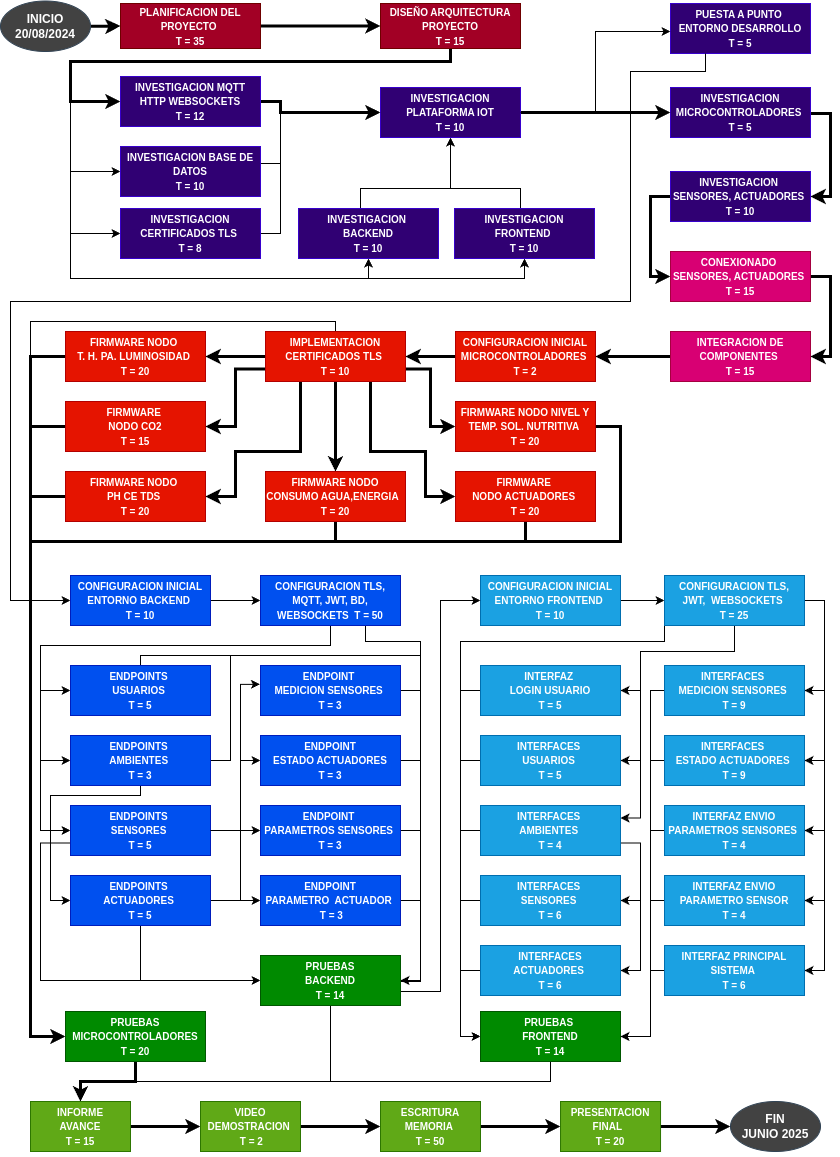
\includegraphics[width=.8\textwidth]{./Figuras/AoN.png}
		\caption{Diagrama de \textit{Activity on Node}.}
		\label{fig:AoN}
	\end{figure}

	Indicar claramente en qué unidades están expresados los tiempos.
	De ser necesario indicar los caminos semi críticos y analizar sus tiempos mediante un cuadro.
	Es recomendable usar colores y un cuadro indicativo describiendo qué representa cada color.

\end{consigna}

\section{11. Diagrama de Gantt}
\label{sec:gantt}

\begin{consigna}{red}
	Existen muchos programas y recursos \textit{online} para hacer diagramas de Gantt, entre los cuales destacamos:

	\begin{itemize}
		\item Planner
		\item GanttProject
		\item Trello + \textit{plugins}. En el siguiente link hay un tutorial oficial: \\ \url{https://blog.trello.com/es/diagrama-de-gantt-de-un-proyecto}
		\item Creately, herramienta online colaborativa. \\\url{https://creately.com/diagram/example/ieb3p3ml/LaTeX}
		\item Se puede hacer en latex con el paquete \textit{pgfgantt}\\ \url{http://ctan.dcc.uchile.cl/graphics/pgf/contrib/pgfgantt/pgfgantt.pdf}
	\end{itemize}

	Pegar acá una captura de pantalla del diagrama de Gantt, cuidando que la letra sea suficientemente grande como para ser legible.
	Si el diagrama queda demasiado ancho, se puede pegar primero la ``tabla'' del Gantt y luego pegar la parte del diagrama de barras del diagrama de Gantt.

	Configurar el software para que en la parte de la tabla muestre los códigos del EDT (WBS).\\
	Configurar el software para que al lado de cada barra muestre el nombre de cada tarea.\\
	Revisar que la fecha de finalización coincida con lo indicado en el Acta Constitutiva.

	En la figura \ref{fig:gantt}, se muestra un ejemplo de diagrama de gantt realizado con el paquete de \textit{pgfgantt}.
	En la plantilla pueden ver el código que lo genera y usarlo de base para construir el propio.

	Las fechas pueden ser calculadas utilizando alguna de las herramientas antes citadas. Sin embargo, el siguiente ejemplo
	fue elaborado utilizando
	\href{https://docs.google.com/spreadsheets/d/1fBz8NhSpc4tkkhz3KjJCbh1nR_ltDkfEcZi4tZXduqs}{esta hoja de cálculo}.

	Es importante destacar que el ancho del diagrama estará dado por la longitud del texto utilizado para las tareas
	(Ejemplo: tarea 1, tarea 2, etcétera) y el valor \textit{x unit}. Para mejorar la apariencia del diagrama, es necesario
	ajustar este valor y, quizás, acortar los nombres de las tareas.

	\begin{figure}[htpb]
		\begin{center}
			\begin{ganttchart}[
					time slot unit=day,
					time slot format=isodate,
					x unit=0.038cm,
					y unit title=0.7cm,
					y unit chart=0.6cm,
					milestone/.append style={xscale=4}
				]{2021-03-05}{2021-12-16}
				\gantttitlecalendar*{2021-03-05}{2021-12-16}{year} \\
				\gantttitlecalendar*{2021-03-05}{2021-12-16}{month} \\
				\ganttgroup{Duración Total}{2021-03-05}{2021-12-16} \\
				%%%%%%%%%%%%%%%%%Organización
				\ganttgroup{Organización}{2021-03-05}{2021-04-16} \\
				\ganttbar{Planificación del proyecto}{2021-03-05}{2021-04-15} \\
				%%%%%%%%%%%%%%%%%Ejecución
				\ganttgroup{Ejecución}{2021-04-16}{2021-10-21} \\
				\ganttbar{Tarea 1}{2021-04-16}{2021-04-29} \\
				\ganttbar{Tarea 2}{2021-04-30}{2021-05-13} \\
				\ganttbar{Tarea 3}{2021-05-14}{2021-05-27} \\
				\ganttbar{Tarea 4}{2021-05-28}{2021-07-12} \\
				\ganttbar{Tarea 5}{2021-07-13}{2021-08-09} \\
				\ganttbar{Tarea 6}{2021-08-10}{2021-09-23} \\
				\ganttbar{Tarea 7}{2021-09-24}{2021-09-30} \\
				\ganttbar{Tarea 8}{2021-10-01}{2021-10-14} \\
				\ganttbar{Tarea 9}{2021-10-15}{2021-10-21} \\
				% %%%%%%%%%%%%%%%%%Finalización
				\ganttgroup{Finalización}{2021-10-22}{2021-12-16} \\
				\ganttbar{Memoria v1}{2021-10-22}{2021-11-04} \\
				\ganttbar{Memoria v2}{2021-11-05}{2021-11-18} \\
				\ganttbar{Memoria final}{2021-11-19}{2021-12-02} \\
				% La fecha del siguiente milestone es la fecha en que terminamos la memoria
				\ganttmilestone{Enviar memoria al director}{2021-12-02} \\
				\ganttbar{Elaborar la presentación}{2021-12-03}{2021-12-16} \\
				\ganttmilestone{Ensayo de la presentación}{2021-12-16} \\
				%%%%%%%%%%%%%%%%%%%%%%%%%%%%%%%%%%%%%%%%%%%%%%%%%%%%%%%%%%%%%%%
			\end{ganttchart}
		\end{center}
		\caption{Diagrama de gantt de ejemplo}
		\label{fig:gantt}
	\end{figure}


	\begin{landscape}
		\begin{figure}[htpb]
			\centering
			\includegraphics[height=.85\textheight]{./Figuras/Gantt-2.png}
			\caption{Ejemplo de diagrama de Gantt (apaisado).} %Modificar este título acorde.
			\label{fig:diagGantt}
		\end{figure}

	\end{landscape}

\end{consigna}


\section{12. Presupuesto detallado del proyecto}
\label{sec:presupuesto}

\begin{consigna}{red}
	Si el proyecto es complejo entonces separarlo en partes:
	\begin{itemize}
		\item Un total global, indicando el subtotal acumulado por cada una de las áreas.
		\item El desglose detallado del subtotal de cada una de las áreas.
	\end{itemize}

	IMPORTANTE: No olvidarse de considerar los COSTOS INDIRECTOS.

	Incluir la aclaración de si se emplea como moneda el peso argentino (ARS) o si se usa moneda extranjera (USD, EUR, etc). Si es en moneda extranjera se debe indicar la tasa de conversión respecto a la moneda local en una fecha dada.

\end{consigna}

\begin{table}[htpb]
	\centering
	\begin{tabularx}{\linewidth}{@{}|X|c|r|r|@{}}
		\hline
		\rowcolor[HTML]{C0C0C0}
		\multicolumn{4}{|c|}{\cellcolor[HTML]{C0C0C0}COSTOS DIRECTOS}   \\ \hline
		\rowcolor[HTML]{C0C0C0}
		Descripción                                                 &
		\multicolumn{1}{c|}{\cellcolor[HTML]{C0C0C0}Cantidad}       &
		\multicolumn{1}{c|}{\cellcolor[HTML]{C0C0C0}Valor unitario} &
		\multicolumn{1}{c|}{\cellcolor[HTML]{C0C0C0}Valor total}        \\ \hline
		                                                            &
		\multicolumn{1}{c|}{}                                       &
		\multicolumn{1}{c|}{}                                       &
		\multicolumn{1}{c|}{}                                           \\ \hline
		                                                            &
		\multicolumn{1}{c|}{}                                       &
		\multicolumn{1}{c|}{}                                       &
		\multicolumn{1}{c|}{}                                           \\ \hline
		\multicolumn{1}{|l|}{}                                      &
		                                                            &
		                                                            &
		\\ \hline
		\multicolumn{1}{|l|}{}                                      &
		                                                            &
		                                                            &
		\\ \hline
		\multicolumn{3}{|c|}{SUBTOTAL}                              &
		\multicolumn{1}{c|}{}                                           \\ \hline
		\rowcolor[HTML]{C0C0C0}
		\multicolumn{4}{|c|}{\cellcolor[HTML]{C0C0C0}COSTOS INDIRECTOS} \\ \hline
		\rowcolor[HTML]{C0C0C0}
		Descripción                                                 &
		\multicolumn{1}{c|}{\cellcolor[HTML]{C0C0C0}Cantidad}       &
		\multicolumn{1}{c|}{\cellcolor[HTML]{C0C0C0}Valor unitario} &
		\multicolumn{1}{c|}{\cellcolor[HTML]{C0C0C0}Valor total}        \\ \hline
		\multicolumn{1}{|l|}{}                                      &
		                                                            &
		                                                            &
		\\ \hline
		\multicolumn{1}{|l|}{}                                      &
		                                                            &
		                                                            &
		\\ \hline
		\multicolumn{1}{|l|}{}                                      &
		                                                            &
		                                                            &
		\\ \hline
		\multicolumn{3}{|c|}{SUBTOTAL}                              &
		\multicolumn{1}{c|}{}                                           \\ \hline
		\rowcolor[HTML]{C0C0C0}
		\multicolumn{3}{|c|}{TOTAL}                                 &
		\\ \hline
	\end{tabularx}%
\end{table}


\section{13. Gestión de riesgos}
\label{sec:riesgos}

\begin{consigna}{red}
	a) Identificación de los riesgos (al menos cinco) y estimación de sus consecuencias:

	Riesgo 1: detallar el riesgo (riesgo es algo que si ocurre altera los planes previstos de forma negativa)
	\begin{itemize}
		\item Severidad (S): mientras más severo, más alto es el número (usar números del 1 al 10).\\
		      Justificar el motivo por el cual se asigna determinado número de severidad (S).
		\item Probabilidad de ocurrencia (O): mientras más probable, más alto es el número (usar del 1 al 10).\\
		      Justificar el motivo por el cual se asigna determinado número de (O).
	\end{itemize}

	Riesgo 2:
	\begin{itemize}
		\item Severidad (S): X.\\
		      Justificación...
		\item Ocurrencia (O): Y.\\
		      Justificación...
	\end{itemize}

	Riesgo 3:
	\begin{itemize}
		\item Severidad (S):  X.\\
		      Justificación...
		\item Ocurrencia (O): Y.\\
		      Justificación...
	\end{itemize}


	b) Tabla de gestión de riesgos:      (El RPN se calcula como RPN=SxO)

	\begin{table}[htpb]
		\centering
		\begin{tabularx}{\linewidth}{@{}|X|c|c|c|c|c|c|@{}}
			\hline
			\rowcolor[HTML]{C0C0C0}
			Riesgo & S & O & RPN & S* & O* & RPN* \\ \hline
			       &   &   &     &    &    &      \\ \hline
			       &   &   &     &    &    &      \\ \hline
			       &   &   &     &    &    &      \\ \hline
			       &   &   &     &    &    &      \\ \hline
			       &   &   &     &    &    &      \\ \hline
		\end{tabularx}%
	\end{table}

	Criterio adoptado:

	Se tomarán medidas de mitigación en los riesgos cuyos números de RPN sean mayores a...

	Nota: los valores marcados con (*) en la tabla corresponden luego de haber aplicado la mitigación.

	c) Plan de mitigación de los riesgos que originalmente excedían el RPN máximo establecido:

	Riesgo 1: plan de mitigación (si por el RPN fuera necesario elaborar un plan de mitigación).
	Nueva asignación de S y O, con su respectiva justificación:
	\begin{itemize}
		\item Severidad (S*): mientras más severo, más alto es el número (usar números del 1 al 10).
		      Justificar el motivo por el cual se asigna determinado número de severidad (S).
		\item Probabilidad de ocurrencia (O*): mientras más probable, más alto es el número (usar del 1 al 10).
		      Justificar el motivo por el cual se asigna determinado número de (O).
	\end{itemize}

	Riesgo 2: plan de mitigación (si por el RPN fuera necesario elaborar un plan de mitigación).

	Riesgo 3: plan de mitigación (si por el RPN fuera necesario elaborar un plan de mitigación).

\end{consigna}


\section{14. Gestión de la calidad}
\label{sec:calidad}

\begin{consigna}{red}
	Elija al menos diez requerimientos que a su criterio sean los más importantes/críticos/que aportan más valor y para cada uno de ellos indique las acciones de verificación y validación que permitan asegurar su cumplimiento.

	\begin{itemize}
		\item Req \#1: copiar acá el requerimiento con su correspondiente número.

		      \begin{itemize}
			      \item Verificación para confirmar si se cumplió con lo requerido antes de mostrar el sistema al cliente. Detallar.
			      \item Validación con el cliente para confirmar que está de acuerdo en que se cumplió con lo requerido. Detallar.
		      \end{itemize}

	\end{itemize}

	Tener en cuenta que en este contexto se pueden mencionar simulaciones, cálculos, revisión de hojas de datos, consulta con expertos, mediciones, etc.

	Las acciones de verificación suelen considerar al entregable como ``caja blanca'', es decir se conoce en profundidad su funcionamiento interno.

	En cambio, las acciones de validación suelen considerar al entregable como ``caja negra'', es decir, que no se conocen los detalles de su funcionamiento interno.

\end{consigna}

\section{15. Procesos de cierre}
\label{sec:cierre}

\begin{consigna}{red}
	Establecer las pautas de trabajo para realizar una reunión final de evaluación del proyecto, tal que contemple las siguientes actividades:

	\begin{itemize}
		\item Pautas de trabajo que se seguirán para analizar si se respetó el Plan de Proyecto original:\\
		      - Indicar quién se ocupará de hacer esto y cuál será el procedimiento a aplicar.
		\item Identificación de las técnicas y procedimientos útiles e inútiles que se emplearon, los problemas que surgieron y cómo se solucionaron:\\
		      - Indicar quién se ocupará de hacer esto y cuál será el procedimiento para dejar registro.
		\item Indicar quién organizará el acto de agradecimiento a todos los interesados, y en especial al equipo de trabajo y colaboradores:\\
		      - Indicar esto y quién financiará los gastos correspondientes.
	\end{itemize}

\end{consigna}

\end{document}